\chapter{Die Realisierung}
\label{cha:Realisierung}
Folgendes Kapitel befasst sich mit der Implementierung, der im Kapitel \ref{cha:Lösungskonzept} vorgestellten Spezifikation des Vorlagenmanagements. Die Implementierung wurde in \emph{Java 8} mit dem \emph{Buildtool Maven} realisiert, wobei die Implementierungen in der folgenden Projektstruktur organisiert wurden.
\newline
\dirtree{%
.1 mailing.
.2 module.
.3 template.
.4 cdi.
.4 jsf.
.4 model.
.5 json.
.4 logic.
.5 api.
.5 impl.
.3 integration.
.4 clevercure-web.
.2 testsuite.
.3 cdi.
.2 demo.
.3 web.
.2 data.
.3 api.
.3 impl.
}
\ \newline
Das Wurzelprojekt \emph{mailing} organisiert alle Abhängigkeiten für die Unterprojekte sowie die gemeinsame \emph{Build}-Konfiguration, die auf alle konkreten Projekte angewendet werden kann. Ebenfalls enthält es die Metadaten wie die EntwicklerInnen, die an diesem Projekt mitwirken. Die Unterprojekte, die ebenfalls \emph{Paren}-Projekte bündeln ihre Unterprojekte und organisieren keine Abhängigkeiten und definieren keine Metadaten. Die gesamte Organisation findet im \emph{Paren}-Projekt \emph{mailing} statt. Diese Projektstruktur wurde gewählt, da in diesem Projekt in weitere Folge auch die Implementierungen der anderen benötigten Softwarekomponenten des \emph{Mail-Service} beinhalten wird. Die konkreten Artefakte wurden jeweils in ein Artefakt \emph{*-api} und \emph{*-impl} aufgeteilt, somit sind die Schnittstellen vollständig getrennt von der Implementierung.
\newline
\newline
Die folgenden Artefakte resultieren aus dieser Projektstruktur, wobei nur die konkreten Artefakte und nicht die \emph{Parent}-Artefakte angeführt sind.
\begin{itemize}
	\item\emph{\textbf{mailing-module-template-logic-api}} ist das Artefakt, das die Spezifikation des Vorlagenmanagement enthält.
	\item\emph{\textbf{mailing-module-template-logic-impl}} ist das Artefakt, das die Implementierung der Spezifikation des Vorlagenmanagements enthält.
	\item\emph{\textbf{mailing-module-template-cdi}} ist das Artefakt, das die Implementierung für die Integration in einen \emph{CDI-Container} enthält.
	\item\emph{\textbf{mailing-module-template-jsf}} ist das Artefakt, das die Implementierung für die Integartion in \emph{JSF} enthält.
	\item\emph{\textbf{mailing-module-template-model-json}} ist das Artefakt, das die Implementierung der \emph{JSON}-Spezifikation enthält.
	\item\emph{\textbf{mailing-module-integartion-clevercure-web}} ist das Artefakt, das die Implementierung der Integration für die Anwendung \emph{CleverWeb} enthält.
	\item\emph{\textbf{mailing-data-api}} ist das Artefakt, dass die Spezifikation der \emph{Services} enthält.
	\item\emph{\textbf{mailing-data-impl}} ist das Artefakt, das die Implementierung der \emph{Service}-Spezifikation enthält.
	\item\emph{\textbf{mailing-testsuite-cdi}} ist das Artefakt, das die Basis aller Tests, die in einem \emph{CDI-Container} lauffähig sein sollen darstellt.
	\item\emph{\textbf{mailing-demo-web}} ist das Artefakt, das die Demowebanwendung darstellt.
\end{itemize} 
\ \newline


\section{Die Implementierung der Spezifikationen}
Der folgende Abschnitt behandelt die Implementierungen der im Kapitel \ref{cha:Lösungskonzept} vorgestellten Spezifikation.

\subsection{Die Implementierung für \emph{CKEditor}}
\emph{CKEditor} ist ein \emph{Javascript} basierter mit dem die Vorlagen bearbeitet werden können. Wie in \ref{sec:sub-typescript-javascript} vorgegeben wird ein \emph{Plugin} benötigt, dass innerhalb des \emph{CKEDitor} die Variablen verwalten kann. Diese \emph{Plugin} wurde in \emph{Typescript} implementiert, da hier Typsicherheit vorhanden ist im Gegenzug zu Javascript das nicht typsicher ist. Die Implementierung des \emph{Plugins} in \emph{Typescript} war möglich, da für den \emph{CKEditor} Typinformationen für \emph{Typescript} vom dem \emph{Open-Source} Projekt \emph{DefinitelyTyped} bereitgestellt wird. \emph{Typescript} benötigt Typinformationen für \emph{Javascript} Quelltext, damit die Typsicherheit in \emph{Typescript} gewährleistet werden kann. Würden keine Typinformationen zur Verfügung stehen, hätte man sie selber implementieren müssen. 
\newline
\newline
Der Quelltext befindet sich zurzeit im Projekt \emph{mailing-demo-web}, da die Verwendung eines \emph{Web-Fragment} das Problem mit sich bringt, dass während der Entwicklung die Ressourcen nicht automatisch nachgeladen werden können, was die Entwicklung sehr erschwert. Da es sich aber nur um zwei Quelltexte handelt, die einfach verschoben werden können, stellt das kein Problem dar.
 
\subsubsection{Das \emph{CKEDitor-Plugin} in Typescript}
Da das Variablenmanagement unabhängig vom verwendeten \emph{CKEditor} ist, wurde die Verwaltung der Variablen in einem eigenen \emph{Javascript} Modul \emph{cc.variables} zusammengefasst. Das \emph{CKEditor Plugin} wurde im \emph{Javascript} Modul \emph{cc.ckeditor.plugins} zusammengefasst. Das Variablenmanagement in \emph{Typescript} ist verantwortlich für die \emph{Browser} seitige Registrierung der Variablen und stellt Hilfsmethoden zur Verfügung zur Verfügung, mit denen Variablen in der \emph{Registry} gefunden und konvertiert werden können. Folgendes Beispiel soll illustrieren wie eine Variable konvertiert werden kann.
\begin{JsCode}[numbers=none]
// Signature of the converter function
public convertVariables(converter:(item:VariableMapping) => any 
                        = (item:VariableMapping)=> item):any[]

// Convert to the variable's set displayName
variablesHandler.convertVariables(
	function (variable) {
		return variable.displayName;
	}
)                        
\end{JsCode}
Die Funktion \emph{convertVariables} definiert den Formalparameter \emph{converter} als eine sogenannte \emph{Arrow}-Funktion, die einer \emph{Lambda}-Funktion in \emph{Java} ähnelt. Mit der \emph{Arrow}-Funktion wird die Signatur der Funktion für die Konvertierung vorgegeben. Ebenfalls wird für den Formalparameter \emph{converter} eine Standardimplementierung definiert, die verwendet wird, sollte der Formalparameter \emph{converter} bei Aktivierung der Funktion \emph{convertVariables} nicht gesetzt sein. Der Typ \emph{any[]} ist vergleichbar mit dem Datentyp \emph{var} aus \emph{.NET} und gibt an das jeder Datentyp als Typ des zurückgelieferten \emph{Arrays} erlaubt ist.
\newline
\newline
Das \emph{CKEditor Plugin} ist für die Integration der Variablen in den \emph{Editor} verantwortlich, wobei die zur Verfügung stehenden Variablen über einen Dialog ausgewählt werden können. Ausgewählte Variablen werden an die aktuelle Position des Cursors im \emph{Editor} in Form eines \emph{HTML Tags} platziert. Die \emph{HTML}-Repräsentation der Variable ist gekoppelt an den \emph{FacesConverter}, da der Konverter die Variable von dessen \emph{HTML}-Repräsentation in die \emph{Template-Engine} spezifische Repräsentation überführen können muss. Die verwendete \emph{Template-Engine} ist für diese \emph{Plugin} irrelevant, da die Variablen immer in dieselbe \emph{JSON}-Repräsentation überführt werden.
\begin{figure}[h]
\centering
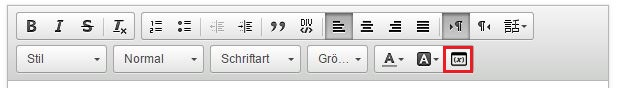
\includegraphics[scale=0.7]{ckeditor-toolbar-open-dialog}
\caption{\emph{CKEditor Toolbar Button} zum Öffnen des Dialogs}
\label{fig:ckeditor-toolbar-opne-dialog}
\end{figure}
\ \newline
Der in Abbildung \ref{fig:ckeditor-toolbar-opne-dialog} rot markierte \emph{Toolbar Button} wird über das \emph{Plugin} registriert und in die \emph{Toolbar} eingefügt. Über diesen \emph{Button} kann der Dialog für die Variablenauswahl geöffnet werden.
\begin{figure}[h]
\centering
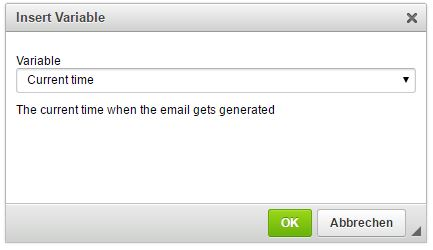
\includegraphics[scale=1]{ckeditor-dialog-insert-variable}
\caption{\emph{CKEditor} Dialog für die Variablenauswahl}
\label{fig:ckeditor-dialog-insert-variable}
\end{figure}
\ \newline
Über den Dialog aus Abbildung \ref{fig:ckeditor-dialog-insert-variable} stehen alle im \emph{CKEditor Plugin} registrierten Variablen zur Auswahl. Der Titel der Variable ist der Text in der Auswahlkomponente und die Beschreibung der ausgewählten Variable wird unterhalb der Auswahlkomponente angezeigt. Durch klick auf den \emph{Button OK} wird die Variable in die Vorlage eingefügt und der Dialog wird geschlossen.
\begin{figure}[h]
\centering
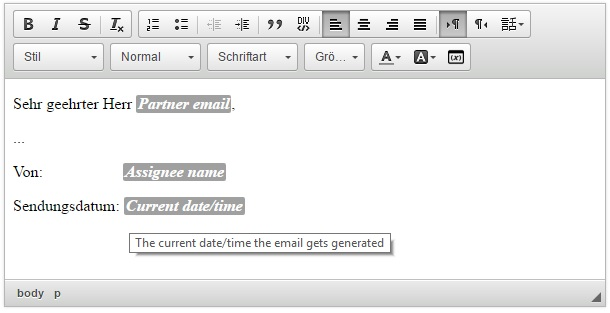
\includegraphics[scale=0.8]{ckeditor-example-template}
\caption{Beispiel einer Vorlage im \emph{CKEditor}}
\label{fig:ckeditor-example-template}
\end{figure}
\ \newline 
Die Abbildung \ref{fig:ckeditor-example-template} illustriert eine Vorlage innerhalb des \emph{CKEditors}, wobei die eingefügten Variablen besonders hervorgehoben werden. Der Titel der Variable stellt den Name für den \emph{HTML Tag} bereit und die Beschreibung dessen Titel. Die eingefügten \emph{HTML Tags} dürfen nicht verändert werden, daher ist das \emph{Drag and Drop} und das Selektieren dieses eingefügten Texts nicht erlaubt, da dadurch die \emph{HTML}-Repräsentation der Variablen zerstört werden könnte und die Variablen nicht mehr vom \emph{FacesConverter} gefunden werden können.
\newpage

\subsubsection{Die Variablenrepräsentation in JSON}
Die Variablen werden als Objekte der Schnittstelle \emph{VariableContract} definiert, und müssen für den \emph{CKEditor} in eine \emph{JSON}-Repräsentation überführt werden, die als \emph{Javascript}-Objekte innerhalb des \emph{CKEDitor Plugins} verwendet werden können. Dafür wurde in \emph{Typescript} eine Schnittstelle definiert, die die Struktur einer Variable innerhalb von \emph{Typescript} und \emph{Javascript} spezifiziert.
\begin{JsCode}[numbers=none]
module cc.variables {

    export interface VariableMapping {
    
        id:string,
        
        displayName:string,
        
        info:string,
    }
    
    ...
}
\end{JsCode}
\ \newline
Diese Schnittstelle ist Teil des Moduls \emph{cc.variables} und wird mit dem Schlüsselwort \emph{export} nach außen offengelegt und kann über den vollständigen Pfad \emph{cc.variables.VariableMapping} innerhalb von \emph{Typescript} und \emph{Javascript} verwendet werden. Mit dieser Schnittstelle werden Typinformationen für \emph{Typescript} bereitgestellt, die innerhalb von \emph{Typescript} die Typsicherheit sicherstellen. Solange die Variablen, die registriert werden, dieser Spezifikation folgen, können innerhalb des \emph{Typescipt} Quelltext keine Fehler auftreten.
\newline
\newline
Der Quelltext aus \ref{prog:variableJson} zeigt die Implementierung der \emph{JSON}-Spezifikation in \emph{Java}, die dazu verwendet wird, die Variablen in den spezifizierten \emph{JSON-String} zu überführen. Damit wird sichergestellt, das die Variablen in \emph{Typescript} korrekt registriert werden. Als \emph{JSON Provider} wird die Bibliothek \emph{fasterxml-jackson-json} vormals \emph{jackson-json} verwendet, die es erlaubt mit Annotationen deklarativ Attribute und/oder Methoden einer Klasse auf \emph{JSON}-Attribute abzubilden. Durch diesen deklarativen Ansatz sind die Attribute und/oder die Methoden einer Klasse entkoppelt von der \emph{JSON}-Spezifikation und können daher abgeändert werden. Nur ein Ändern des Datentyps eines Attributes könnte zu Problemen führen. 
\begin{program}
\caption{VariableJson.java}
\label{prog:variableJson}
\begin{JsCode}
@JsonTypeName(value = "variable-json")
public class VariableJson extends AbstractJsonModel {

    private String id;
    private String label;
    private String info;

    public VariableJson() {
    }

    public VariableJson(String id,
                        String displayName,
                        String tooltip) {
        this.id = id;
        this.label = displayName;
        this.info = tooltip;
    }

    @JsonGetter("id")
    public String getId() {
        return id;
    }

    @JsonSetter("id")
    public void setId(String id) {
        this.id = id;
    }

    @JsonGetter("displayName")
    public String getLabel() {
        return label;
    }

    @JsonSetter("displayName")
    public void setLabel(String label) {
        this.label = label;
    }

    @JsonGetter("info")
    public String getInfo() {
        return info;
    }

    @JsonSetter("info")
    public void setInfo(String info) {
        this.info = info;
    }
    
}
\end{JsCode}
\end{program}
\ \newpage


\subsection{Die Implementierungen für CDI}
Folgender Abschnitt behandelt die Implementierungen für die Integration in einen \emph{CDI Container}. Wie in Abschnitt \ref{sec:sub-template-management-cdi} beschrieben sollen die Variablen automatisch beim start des \emph{CDI Containers} registriert werden, sowie Vorlagenmanagementressourcen kontextabhängig über eine \emph{CDI Producer} zur Verfügung gestellt werden können. 

\subsubsection{Die Vorlagenmanagement \emph{CDI-Extension}}
Um die Variablen beim Start des \emph{CDI Containers} automatisch registrieren zu können, wurde die Klasse \emph{TemplateCdiExtension} implementiert, die in der Lage ist auf Lebenszyklus \emph{Events} des \emph{CDI -Containers} zu reagieren und die Schnittstelle \emph{javax.enterprise.inject.spi.Extension} implementiert. Die Schnittstelle \emph{javax.enterprise.inject.spi.Extension} enthält keine abstrakten Methoden und markiert ein Implementierung als eine \emph{CDI-Extension}. Die \emph{CDI-Extension} wird als \emph{Service Provider} über die Schnittstelle \emph{Service-Provider-Interface} (SPI) registriert, in dem man eine folgende Datei erstellt \emph{META-INF/services/javax.enterprise.inject.spi.Extension}, die eine normale Textdatei ist und den vollständigen Namen der \emph{Service Provider} Implementierung enthält. 
\newline
\newline
Eine \emph{CDI-Extension} ist eigentlich kein \emph{CDI-Bean}, da ein Objekt der \emph{CDI-Extension} bereits beim Start des \emph{CDI-Containers} erstellt wird und somit existiert bevor der \emph{CDI-Container} vollständig gestartet ist. Trotzdem ist eine Extension injizierbar und kann in \emph{CDI-Beans} injiziert werden. Das erstellte Objekt der \emph{CDI-Extension} existiert über die Lebensdauer des \emph{CDI-Containers}.
\newline
\newline
Das folgende Programm \ref{prog:templateCdiExtension} ist ein Auszug aus der implementierten \emph{CDI-Extension} und illustriert die \emph{CDI-Container} Lebenszyklus \emph{Events}, auf die reagiert wird. Über diese \emph{CDI-Extension} werden alle implementierten Typen der Schnittstelle \emph{VariableContract} gefunden und im Objekt der Klasse \emph{TemplateConfiguration} registriert. Vorerst werden nur Implementierungen der Schnittstelle \emph{VariableContract} unterstützt, die mit dem \emph{Java}-Typ \emph{enum} implementiert wurden. Ebenfalls werden alle implementierten Typen der Schnittstelle \emph{VariableResolverFactory} gefunden und in der \emph{Extension} registriert. Die \emph{Extension} wird  in der später vorgestellten \emph{CDI-Producer} Implementierung verwendet um Objekte der Schnittstelle \emph{VariableResolverFactory} zu produzieren. 
\newpage
\begin{program}[h]
\caption{TemplateCdiExtension.java}
\label{prog:templateCdiExtension}
\begin{JavaCode}
public class TemplateCdiExtension implements Extension,
        Serializable {

    private TemplateConfiguration templateConfig;
    private Map<Class<? extends VariableContract>, 
                Class<VariableResolverFactory>>  
            variableResolverFactoryMap;
    private Logger log;

    void beforeBeanDiscovery(@Observes BeforeBeanDiscovery bbd) {
        // Init class members
    }

    <T> void processCdiVariableContracts
             (@Observes @WithAnnotations({BaseName.class, 
                                          CdiVariableContract.class}) 
             ProcessAnnotatedType<T> pat) {
       // Collect VariableContract implementations (Enum type only)
    }

    <T> void processVariableResolverFactoryFactories
        (@Observes @WithAnnotations(CdiVariableResolverFactory.class) 
        ProcessAnnotatedType<T> pat) {
        // Collect VariableResolverFactory implementations
    }

    // Getter for class members templateConfig
    // and variableResolverFactoryMap
}
\end{JavaCode}
\end{program}
\begin{itemize}
	\item\emph{void beforeBeanDiscovery(...)} 
	\newline
	ist die \emph{Observer}-Methode, die einmalig aufgerufen wird bevor mit dem Auffinden der \emph{CDI-Beans} begonnen wird. In dieser Methode wird die Extension initialisiert.
	\item\emph{<T> void processCdiVariableContracts(...)} 
	\newline
	ist die \emph{Observer}-Methode, die für jeden annotierten Typ aufgerufen wird, der mit den Annotationen \emph{@BaseName} und \emph{@CdiVariableContract} annotiert ist.
	\item\emph{<T> void processVariableResolverFactoryFactories(...)} 
	\newline
	ist die \emph{Observer}-Methode, die für jeden annotierten Typ aufgerufen wird, der mit den Annotationen \emph{@CdiVariableResolverFactory} annotiert ist.
\end{itemize}
\ \newpage

\subsubsection{Der Vorlagenmanagement \emph{CDI-Producer}}
Es wurde ein \emph{CDI-Producer} \emph{TemplateResourceProducer} implementiert, mit dem kontextabhängig Ressourcen des Vorlagenmanagements produziert werden können. Diese Klasse ist die einzige Klasse, die sich die \emph{Extension TemplateCdiExtension} injizieren lässt. Es kann nicht verhindert werden, dass andere \emph{CDI-Beans} sich diese Klasse injizieren, da eine \emph{CDI-Extension}-Klasse öffentlich sein muss. Da mehrere \emph{Template-Engines} unterstützt werden sollen, wurde die Annotation \emph{@FreemarkerTemplate} eingeführt, die einen Injektionspunkt für \emph{Freemarker} qualifiziert. Ebenso wurde jeweils eine \emph{Producer}-Methode für den Qualifizierer \emph{@Default} implementiert, über die Standardimplementierung bereitgestellt wird, die in der derzeitigen Implementierung Implementierungen die den Qualifizierer \emph{@FreemarkerTemplate} produziert. Damit ist sichergestellt, dass keine \emph{UnsatisfiedResolutionException} auftreten kann, obwohl man sich der Gefahr aussetzt, dass die produzierte \emph{@Default} Implementierung nicht die gewollte ist.
\begin{program}[h]
\caption{TemplateResourceProducer.java}
\label{prog:templateResourceProducer}
\begin{JavaCode}
@ApplicationScoped
public class TemplateResourceProducer implements Serializable {
    @Produces
    @ApplicationScoped
    @Default
    public VariableConfiguration produceConfiguration() {
        return extension.getVariableConfiguration();
    }
    
    @Produces
    @Dependent
    @Default
    public TemplateDataJsonBuilder produceDefaultTemplateBuilder
          (final @Default VariableResolverFactoryProvider factory) {
        return produceFreeMarkerTemplateBuilder(factory);
    }

    @Produces
    @Dependent
    @FreemarkerTemplate
    public TemplateDataJsonBuilder produceFreeMarkerTemplateBuilder
           (final @Default VariableResolverFactoryProvider factory) {
        return new FreemarkerTemplateDataJsonBuilder()
                .withWeakMode()
                .withVariableResolverFactoryProvider(factory);
    }
}
\end{JavaCode}
\end{program}
\ \newline
Der Quelltext aus \ref{prog:templateResourceProducer} ist ein Auszug aus der Klasse \emph{TemplateResourceProducer} und dient als Beispiel für die implementierten \emph{Producer}-Methoden. Die beiden implementierten \emph{Producer}-Methoden \emph{produceDefaultTemplateBuilder} und \emph{produceFreeMarkerTemplateBuilder} produzieren Objekte der Schnittstelle \emph{TemplateDataJsonBuilder} für verschiedene Qualifizierer. Die Methode \emph{produceDefaultTemplateBuilder} produziert Objekte der Schnittstelle \emph{TemplateDataJsonBuilder} qualifiziert mit \emph{@Default}, wobei ein Injektionspunkt diesen Qualifizierer nicht explizit angeben muss, da dieser als Standard verwendet wird. Die Methode \emph{produceFreeMarkerTemplateBuilder} produziert Objekte der Schnittstelle \emph{TemplateDataJsonBuilder} qualifiziert mit \emph{@FreemarkerTemplate}, wobei ein Injektionspunkt diesen Qualifizierer explizit angeben muss.  Beide Methoden produzieren Objekte für den sogenannten Pseudo-\emph{Scope @Dependent}, wobei für jeden Injektionspunkt ein neues Objekt erstellt wird.
Als Argument für diesen beiden Methoden wird ein Objekt der Schnittstelle \emph{VariableResolverFactoryProvider} injiziert, der \emph{@Default} qualifiziert ist. Dieses Objekt wird kontextabhängig injiziert, wobei der Geltungsbereich dieses Objekts für die Methoden nicht bekannt ist. 
\newline
\newline
Die Methode \emph{produceConfiguration} produziert ein Objekt der Schnittstelle  \emph{VariableConfiguration}, die die registrierten Variablen enthält und von der \emph{Extension} bereitgestellt wird. Nachdem diese Schnittstelle nur lesenden Zugriff erlaubt und nur die \emph{Extension} Variablen registriert, wird dieses Objekt für den Gültigkeitsbereich der Anwendung produziert, als einmalig für die gesamte Anwendungslaufzeit.

\subsubsection{Die Vorlagenmanagement \emph{CDI-Utility}}
Die Klasse \emph{CdiTemplateUtil} wurde implementiert um ein kontextabhängiges \emph{CDI-Bean} zur Verfügung zu stellen, das Hilfsmethoden für die Konvertierung und Lokalisierung der Variablen bereitstellt. Für die Lokalisierung wurde die Schnittstelle \emph{VariableLocaleProvider} spezifiziert, dessen Implementierung kontextabhängig als \emph{CDI-Bean} zur Verfügung gestellt wird, um ein Objekt der Klasse \emph{java.util.Locale} zu bekommen, dass für die Lokalisierung benötigt wird. Eine Implementierung der Schnittstelle \emph{VariableLocaleProvider} kann dabei das Objekt der Klasse \emph{java.util.Locale} abhängig von einem eingeloggten BenutzerIn bereitstellen, in einem beliebigen Gültigkeitsbereich.
\newline
\newline
Es wird die Implementierung \emph{DefaultVariableLocaleProvider} der Schnittstelle \emph{VariableLocaleProvider} bereitgestellt, die mit \emph{@ApplicationScoped} qualifiziert ist und die das Objekt der Klasse \emph{java.util.Locale} über \emph{Locale.getDefault();} bereitstellt. Diese Implementierung stellt die Standardimplementierung dar. Um eine eigene Implementierung zur Verfügung zu stellen, stehen folgende Möglichkeiten zur Verfügung.
\begin{itemize}
	\item\emph{Spezialisierung} ist eine Möglichkeit ein \emph{Bean} zu spezialisieren, wobei die eigene Implementierung von der spezialisierten Implementierung ableiten und mit \emph{@Specializes} annotiert werden muss. Oder es gibt eine \emph{Producer}-Methode, die mit \emph{@Specializes} annotiert ist. Mit diesem Ansatz werden alle gesetzten Qualifizierer, der Name und der Gültigkeitsbereich geerbt. Die spezialisierte Implementierung wird mit der Spezialisierung deaktiviert und steht nicht mehr zur Verfügung.
	\item\emph{Alternative Implementierung} ist die Möglichkeit für den Typ, in diesem Fall \emph{VariableLocaleProvider}, eine alternative Implementierung zur Verfügung zu stellen, wobei die alternative Implementierung in der \emph{beans.xml} registriert und/oder mit \emph{@Alternative} annotiert werden muss (Abhängig von der konkreten \emph{CDI}-Implementierung). Mit diesem Ansatz kann ein unterschiedlicher Gültigkeitsbereich, Name und Qualifizierer verwendet werden. Mit einer alternativen Implementierung kann die andere Implementierung noch immer zur Verfügung stehen, abhängig ob die Qualifizierer der beiden Implementierungen gleich sind.
\end{itemize}

\subsection{Die Implementierungen für JSF}
Folgender Abschnitt behandelt die Implementierung des Variablenmanagements für die \emph{View}-Technologie \emph{JSF}. In diesem Abschnitt wird sich nur dem implementierten \emph{FacesConverter} und die \emph{CKEditor}-Integration, bereitgestellt von \emph{primefaces-extensions}, beschäftigen.

\subsubsection{Der Vorlagen \emph{FacesConverter}}
Der \emph{FacesConverter} wurde als abstrakte Klasse \emph{AbstractTemplateConverter} implementiert, die die Schnittstelle \emph{javax.faces.Converter} implementiert. Diese abstrakte Klasse wurde implementiert, da die Konvertierungslogik über alle \emph{Template-Engines} dieselbe ist und lediglich sich die Implementierung der Schnittstelle \emph{TemplateProcessor} unterschiedet. Das Objekt der Schnittstelle \emph{TemplateProcessor} und das Objekt der Klasse \emph{CdiTemplateUtil} werden vom \emph{CDI-Container} bereitgestellt, wobei diese Objekte manuell geholt werden müssen, da keine Injektion innerhalb eines \emph{FacesCovnerters} möglich ist. Die Objekte werden über die Klasse \emph{BeanProvider} der Bibliothek \emph{Deltaspike} geholt. \emph{Deltaspike} ist eine Bibliothek, die portable \emph{CDI-Exntensions} bereitstellt. Die konkrete Implementierung \emph{FreemarkerTemplateConverter}, die von der abstrakten Klasse \emph{AbstractTemplateConverter} ableitet, setzt über einen Konstruktor in der Basisklasse den korrespondierenden Qualifizierer für die verwendete \emph{Template-Engine}, um mit diesem Qualifizierer die korrekte Implementierung der Schnittstelle \emph{TemplateProcessor} aus dem \emph{CDI-Container} zu holden.
\newpage
\begin{program}
\caption{FreemarkerTemplateConverter.java}
\label{prog:freemarkerTemplateConverter}
\begin{JavaCode}
@FacesConverter("template.converter.freemarker")
public class FreemarkerTemplateConverter extends AbstractTemplateConverter {

    public FreemarkerTemplateConverter() {
        super(new FreemarkerTemplateLiteral());
    }
}
\end{JavaCode}
\end{program}
\ \newline
Der Quelltext in \ref{prog:freemarkerTemplateConverter} ist die implementierte Klasse für die \emph{Template-Engine Freemarker}. Die Annotation \emph{@FacesConverter("template.converter.freemarker")} definiert einen eindeutigen Namen für diesen Konverter, der in \emph{xhtml} Dateien als Konverter definiert werden kann. Das \emph{JSF-Framework} erstellt dann ein Objekt dieser Klasse für die \emph{JSF}-Komponente, die diesen Konverter verwendet. 

%\subsubsection{Die \emph{Primefaces-Extension} für den \emph{CKEditor}}


%\section{Die Vorlagen-\emph{Management} Beispielanwendung}
%\subsection{Die Verwendung in einem \emph{Business}-Service}
%\subsection{Die Verwendung in der \emph{Web}-Oberfläche}